\documentclass{article}
\usepackage[utf8]{inputenc} %кодировка
\usepackage[T2A]{fontenc}
\usepackage[english,russian]{babel} %русификатор 
\usepackage{mathtools} %библиотека матеши
\usepackage[left=1cm,right=1cm,top=2cm,bottom=2cm,bindingoffset=0cm]{geometry} %изменение отступов на листе
\usepackage{amsmath}
\usepackage{graphicx} %библиотека для графики и картинок
\graphicspath{}
\DeclareGraphicsExtensions{.pdf,.png,.jpg}
\usepackage{subcaption}
\usepackage{pgfplots}
\usepackage{float}
\usepackage{hyperref}

\begin{document}
% НАЧАЛО ТИТУЛЬНОГО ЛИСТА
\begin{center}
    \Large
    Федеральное государственное автономное \\
    образовательное учреждение высшего образования \\ 
    «Научно-образовательная корпорация ИТМО»\\
    \vspace{0.5cm}
    \large
    Факультет программной инженерии и компьютерной техники \\
    Направление подготовки 09.03.04 Программная инженерия \\
    \vspace{1cm}
    \Large
    \textbf{Отчёт по лабораторной работе №1} \\
    По дисциплине «Информационные системы» ( семестр 5)\\
    \large
    \vspace{8cm}

    \begin{minipage}{.33\textwidth}
    \end{minipage}
    \hfill
    \begin{minipage}{.4\textwidth}
    
        \textbf{Студент}: \vspace{.1cm} \\
        \ Дениченко Александр P3312\\
        \textbf{Практик}:  \\
        \ 
    \end{minipage}
    \vfill
Санкт-Петербург\\ 2024 г.
\end{center}
\pagestyle{empty}
% КОНЕЦ ТИТУЛЬНОГО ЛИСТА 
\newpage
\pagestyle{plain}

\section*{Задание}
\begin{center}
    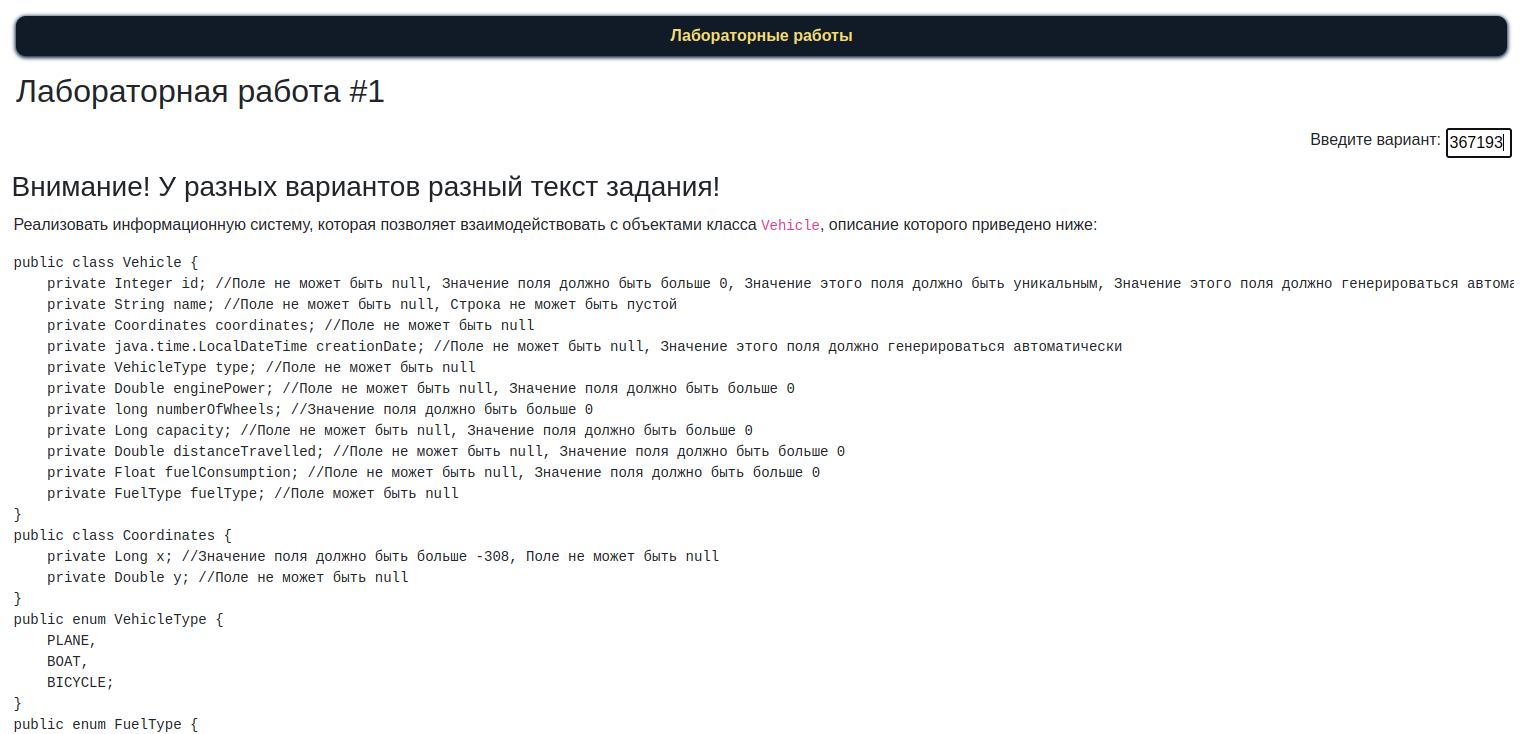
\includegraphics[width=.9\textwidth]{11}
\end{center}
\begin{center}
    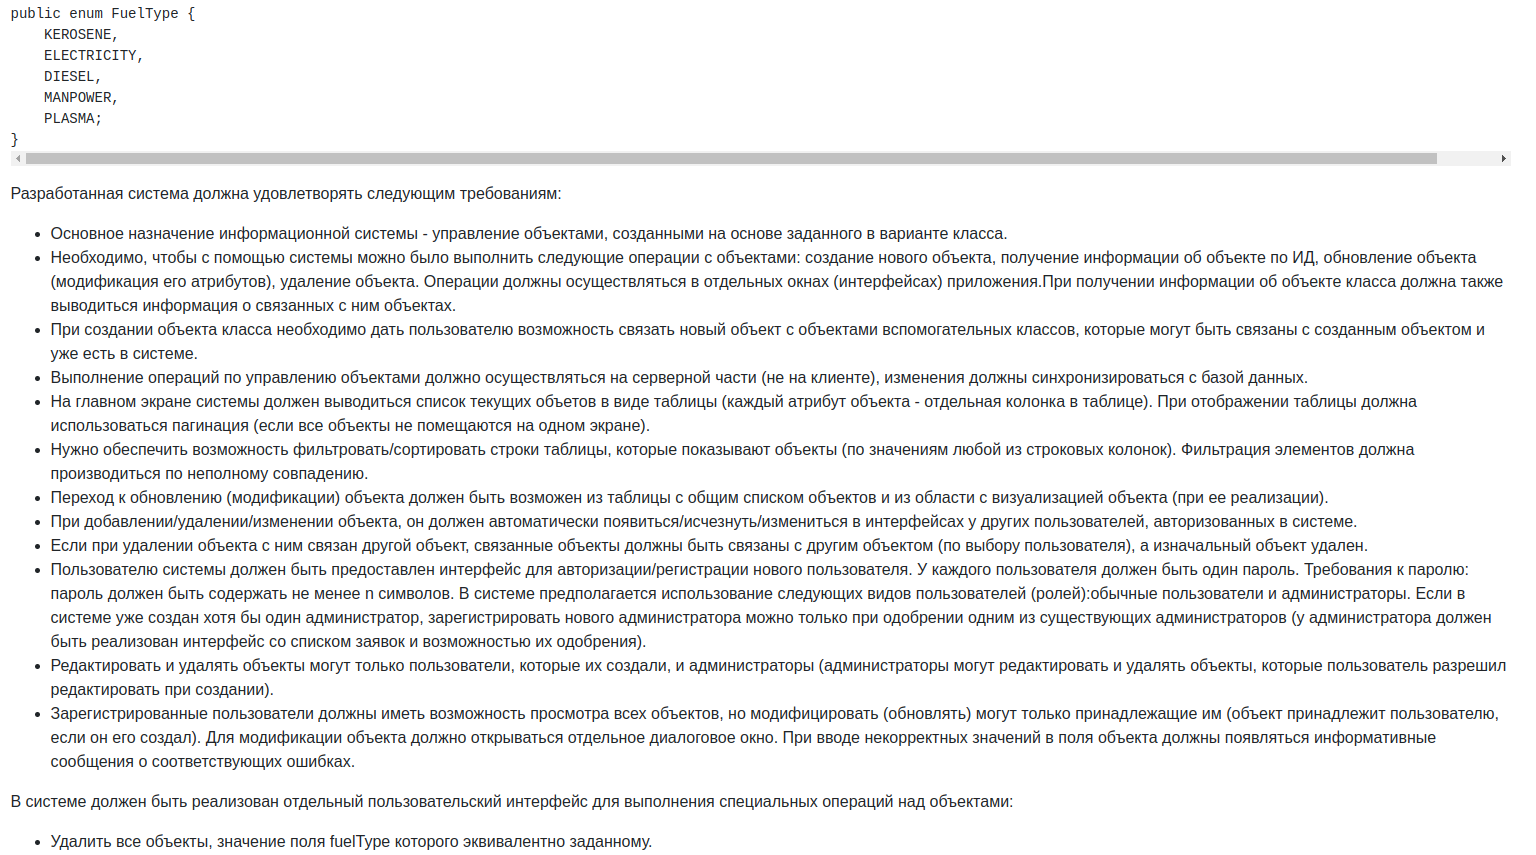
\includegraphics[width=.9\textwidth]{2}
\end{center}
\begin{center}
    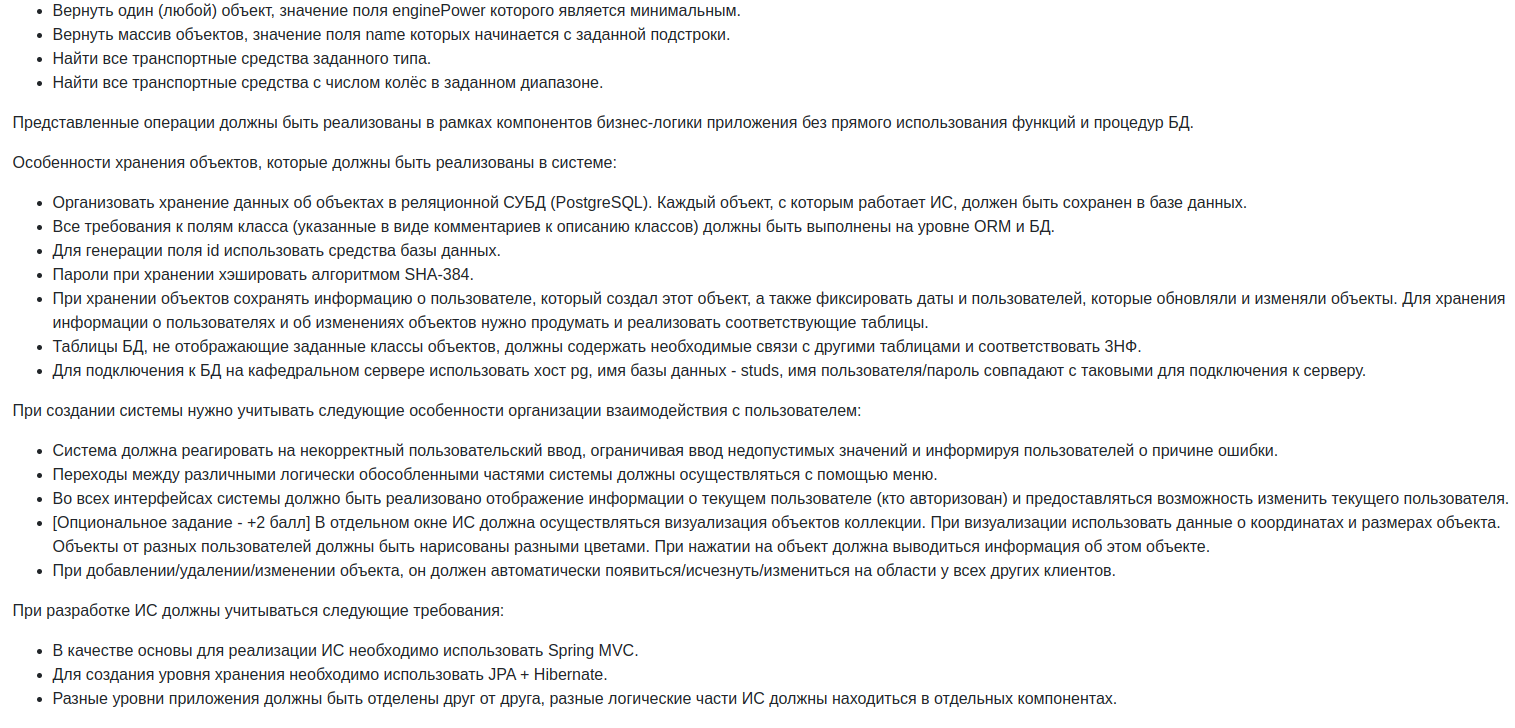
\includegraphics[width=.9\textwidth]{3}
\end{center}

\section{UML диаграммы}
    \subsection{Диаграмма пакетов}
        \begin{center}
            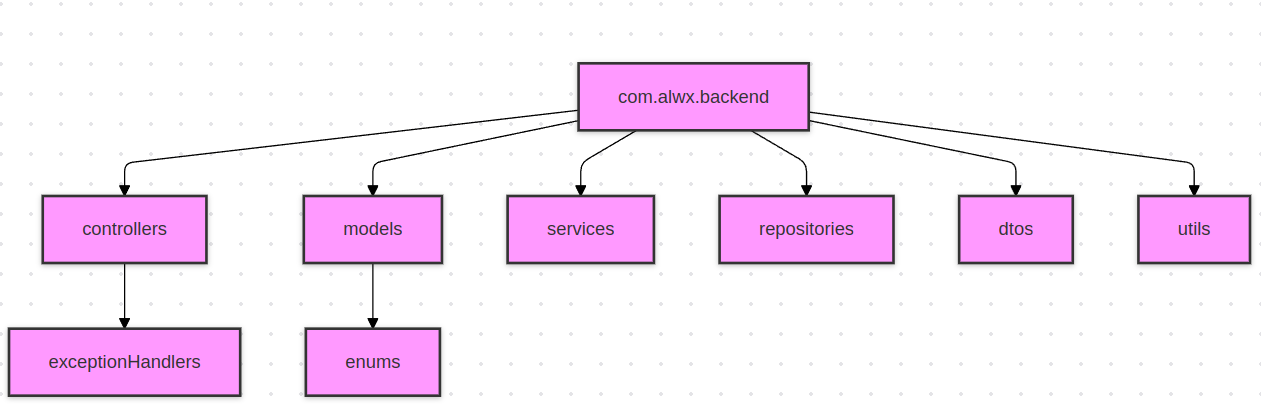
\includegraphics[width=.9\textwidth]{package_uml.png}
        \end{center}

\subsection{Диаграмма классов}
\href{https://www.mermaidchart.com/raw/7b97b9f2-bd1a-4381-be9d-0ba2c8f43344?theme=light&version=v0.1&format=svg}{Ссылка на диаграмму классов}

\section{Ссылка на проект}
\href{https://github.com/DenichenkoAlex/inf_sys_first_lab}{Ссылка на проект}

\section{Доказательство 3НФ формы таблиц базы данных}
1. User:

Ключ: id (простой ключ).

Атрибуты: id, username, password. Все атомарные.

Связь с Role: реализована через отдельную таблицу users\_roles, что соответствует принципам нормализации.
\\
Вывод: User в 3НФ, так как у него простой ключ и нет транзитивных зависимостей.
\\ \\
2. Role:

Ключ: id (простой ключ).

Атрибуты: id, name. Все атомарные.
\\
Вывод: Role в 3НФ, так как у него простой ключ и нет транзитивных зависимостей.
\\ \\
3. Vehicle:

Ключ: id (простой ключ).

Атрибуты: id, name, creationDate, type, enginePower, numberOfWheels, capacity, distanceTravelled, fuelConsumption, fuelType, permissionToEdit. Все атомарные.

Связь с Coordinates: coordinates\_id является внешним ключом, ссылающимся на Coordinates. Это функциональная зависимость, но не транзитивная.

Связь с User: реализована через отдельную таблицу vehicle\_user, что соответствует принципам нормализации.
\\
Вывод: Vehicle в 3НФ.
\\\\
4. Coordinates:

Ключ: id (простой ключ).

Атрибуты: id, x, y. Все атомарные.
\\
Вывод: Coordinates в 3НФ.
\\\\
5. UserAction:

Ключ: id (простой ключ).

Атрибуты: id, action, vehicleId, timestamp, user\_id (внешний ключ, ссылающийся на User). Все атомарные.

Зависимости: user\_id -> username (через таблицу User). Это не транзитивная зависимость, так как user\_id часть ключа.
\\
Вывод: UserAction в 3НФ.
\\\\
6. RequestForRights:

Ключ: id (простой ключ).

Атрибуты: id, username. Все атомарные.
\\
Вывод: RequestForRights в 3НФ.

\section{Выводы}
        В ходе выполнения лабораторной работы, были изучены основные принципы проектирования информационный системы, при помощи которой можно управлять некоторым набором объектов. Хранение данных организованно на уровне базы данных, любые действия, связанные с редактирование данных происходят на уровне сервера, без использования функционала базы данных (она помогает структурировать данные и накладывать некоторые ограничения на поля).
        На уровне сервера были разработанны контроллеры, которые обрабатывают запросы пользователей, и перенаправляют управление в сервисы, которые выполняют всю суть редактирования данных и логику приложения. Взаимодействие с базой данных огранизованно через CRUD операции. Для упрощения взаимодействия используется спецификация JPA и её реализация по работе с упаковкой и распаковкой данных Hibernate.
\end{document}
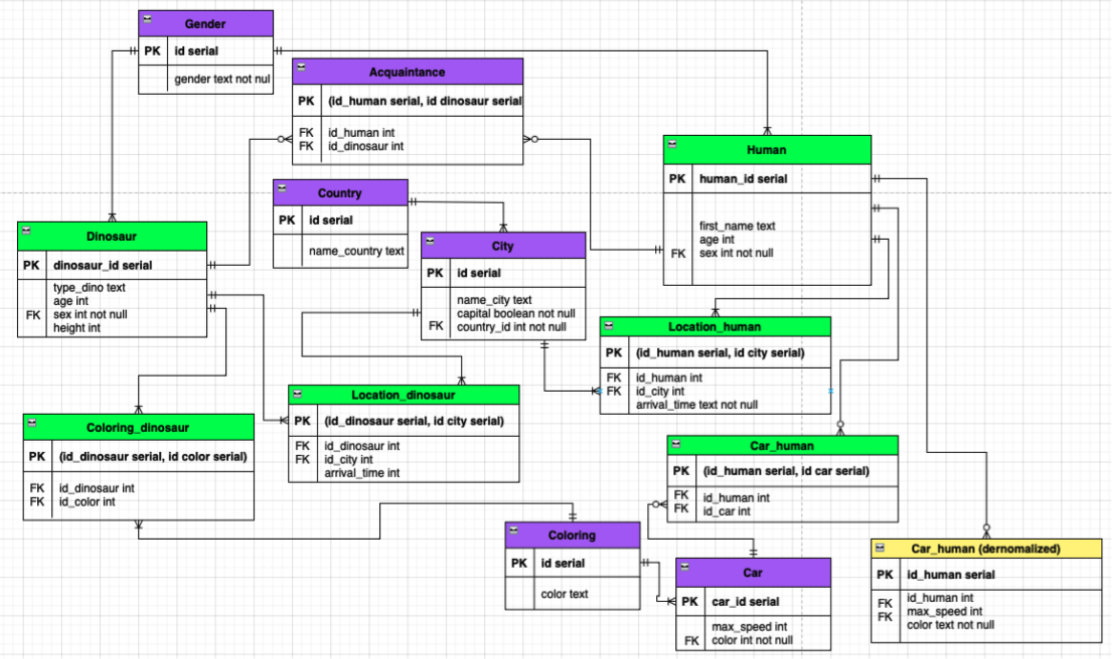
\includegraphics[width=.9\textwidth]{123}